%use in documents with \subfile{tex/intro}
\documentclass[../../master.tex]{subfiles}

\begin{document}

\subsection{Initial Sequence Designs}
\label{sub:appendix:protodesigns}

The figures in this section were included for completeness.
The approach used and the overall performance corresponds to designed sequences of the \texttt{complete} set (cf. \autoref{fig:logos:b} and \ref{fig:stats_constrained}), with the exception that the data from \autoref{fig:azodata:a} was used as reference instead.

\begin{figure}[!ht]
	\centering
	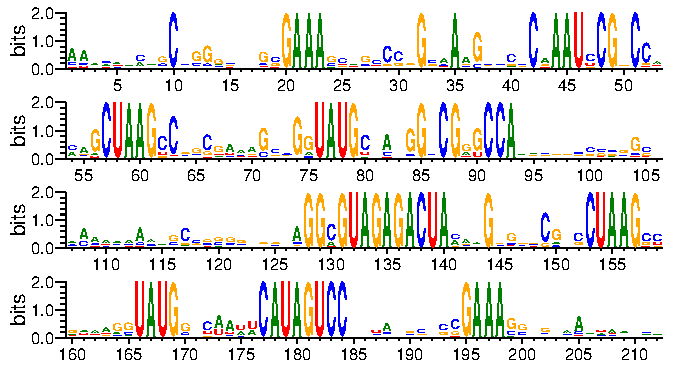
\includegraphics[trim=0 0 0 0, clip, width=0.8\textwidth]{pic/results/designs/logos/logo-proto.pdf}
	\caption[Nucleotide Composition of Initial Constrained Designs]{
		Sequence logo of sequences designed with the \texttt{proto} constraint set ($n = 1000$)
		Nucleotides were colored according to their identity.
		Positions with an information content of \unit[2]{bit} correspond to the sequence constraints.
	}\label{fig:protologo}
\end{figure}


\begin{figure}[!ht]
	\centering
	\begin{subfigure}[t]{0.2\textwidth}
		\centering
		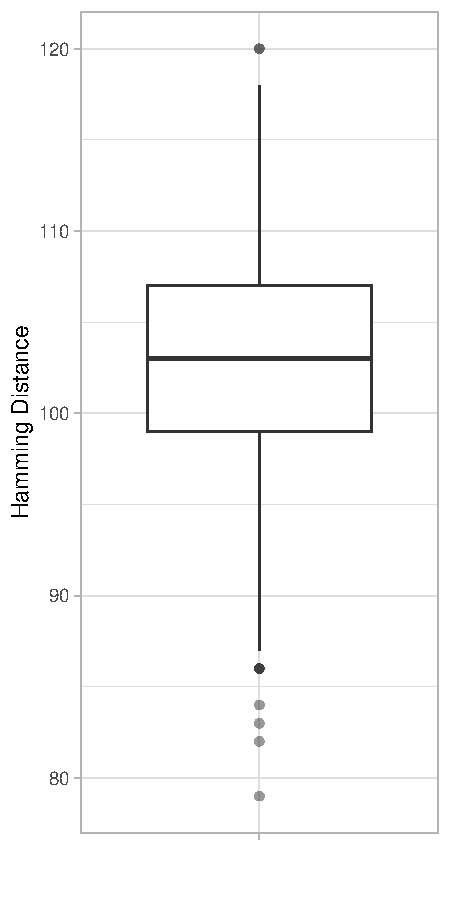
\includegraphics[width=\textwidth]{pic/results/designs/boxplots/proto-hamming-boxplot.pdf}
		\caption{Hamming distance to the native sequence as a measure of sequence similarity.
		}\label{fig:stats_proto:a}
	\end{subfigure}%
	\begin{subfigure}[t]{0.2\textwidth}
		\centering
		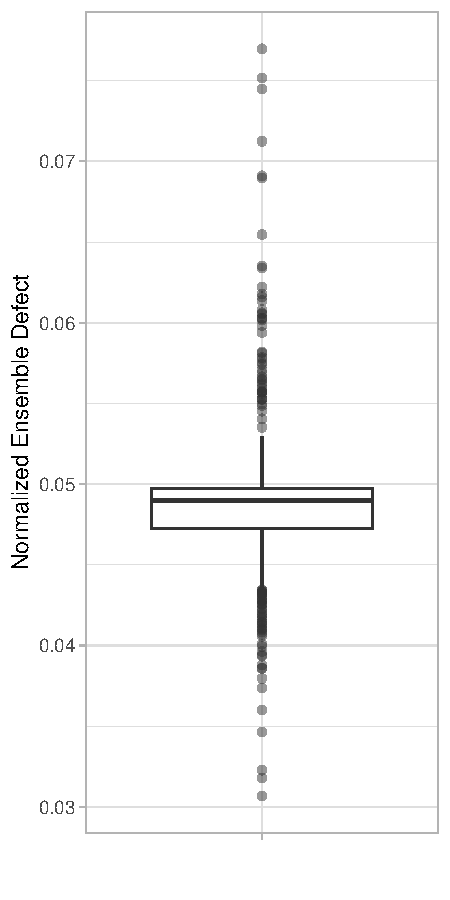
\includegraphics[width=\textwidth]{pic/results/designs/boxplots/proto-score-boxplot.pdf}
		\caption{the normalized ensemble defect to the pseudoknot-free target structure.
		}\label{fig:stats_proto:b}
	\end{subfigure}%
	\begin{subfigure}[t]{0.27\textwidth}
		\centering
		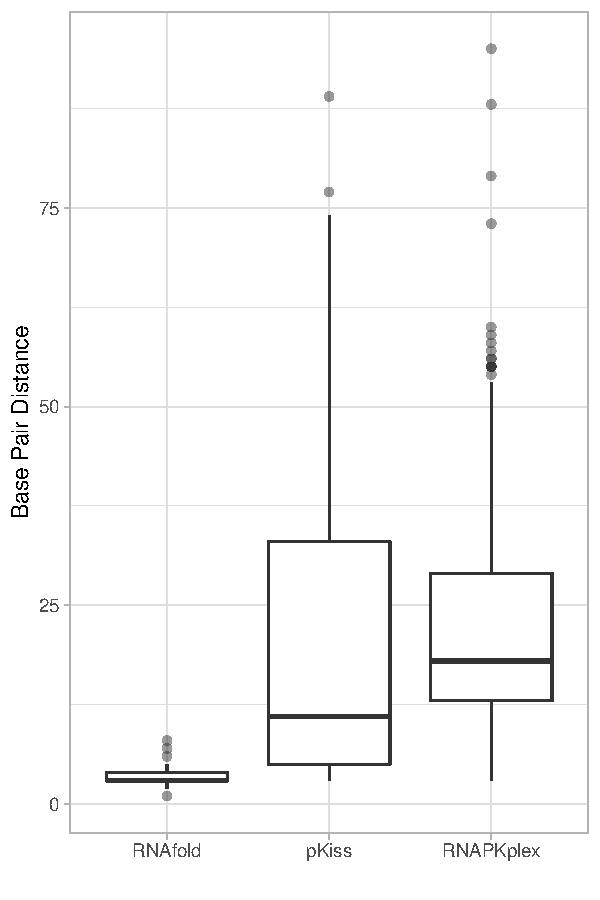
\includegraphics[width=\textwidth]{pic/results/designs/boxplots/proto-bp-boxplot.pdf}
		\caption{Base pair distances relative to the target structure. For predictions made by \texttt{RNAfold}, base pairs of P7 were assumed to be present.
		}\label{fig:stats_proto:c}
	\end{subfigure}
	\begin{subfigure}[t]{0.27\textwidth}
		\centering
		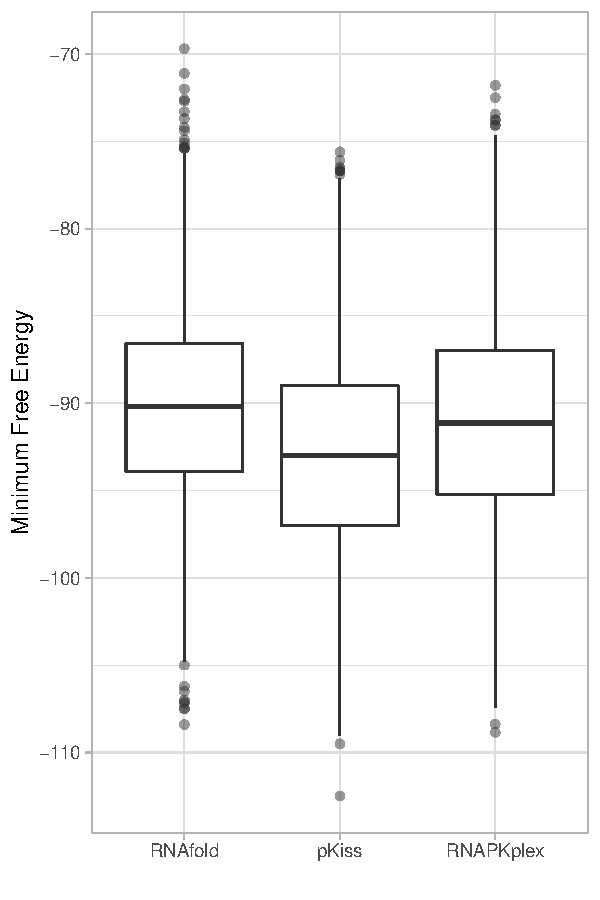
\includegraphics[width=\textwidth]{pic/results/designs/boxplots/proto-mfe-boxplot.pdf}
		\caption{Free Energy of the predicted structures.  \texttt{RNAfold} values were corrected by the energy of the assumed base pairs in P7 (\autoref{fig:p7energy:a}).
		}\label{fig:stats_proto:d}
	\end{subfigure}
	\caption[Properties of Initial Constrained Designs ]{
		Metrics computed for $n = 1000$ sequences designed using the constraint sets \texttt{proto}. Note that computations done by \texttt{RNAfold} or \texttt{ViennaRNA} were subject to structural constraints as described in \autoref{ssub:methods:rnafold}.
		In contrast to Figure \ref{fig:stats_constrained}, the target structure and native reference sequence as seen in \autoref{fig:azodata:a} was used.
	}\label{fig:stats_proto}
\end{figure}

Additionally, these designs did produce base pair probability dot plots with positions corresponding to P7 missing (\autoref{fig:bpp_proto}).

\begin{figure}[!ht]
	\centering
	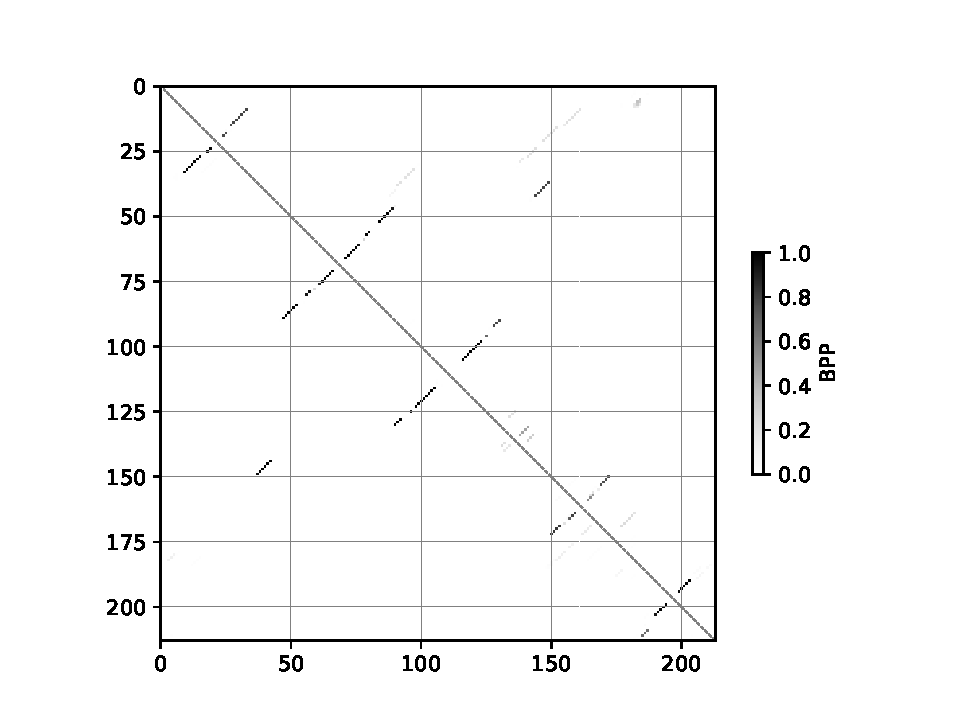
\includegraphics[trim=50 10 50 10, clip, width=0.5\textwidth]{pic/results/designs/dotplots/examples/proto-range.pdf}
	\caption[Base Pair Probabilities of Initial Constrained Designs]{
		Base pair probabilities of two designed sequences, computed using \texttt{ViennaRNA}. Here, the normalized ensemble defect was used as the objective function.
		The lower diagonal half of shows one of the best designs in the \texttt{proto} constraint set according to the average base pair distance of the three MFE predictions used; the upper diagonal half shows one of the worst designs according to the same metric. See \autoref{fig:bpp_pseven:b} for comparison and \autoref{tab:examplefasta} for the exact RNA sequences used here.
	}\label{fig:bpp_proto}
\end{figure}
Based on the average base pair distance of the structures predicted using constrained \texttt{RNAfold}, \texttt{pKiss} and \texttt{RNAPKplex} to the target structure, 10 sequences were selected for preliminary experiments (see \autoref{sub:exp_results}).
These candidates had to be postprocessed for the experimental assays though, which is why for later design runs, the reference data was truncated (\autoref{fig:azodata:b}) and new sequence constraints were added (\autoref{tab:constraintsets}).

\end{document}
